\section{RAID Systeme}
Bei einem \ac{RAID} System werden mehrere Festplatten zu einer großen virtuellen Festplatte zusammengefasst\cite[vgl.][Seite 279 f.]{mandl13}.
Daraus resultiert, dass mindestens zwei Festplatten für den Betrieb eines \ac{RAID}-Systems erforderlich sind.
Solch ein System aus mehreren Festplatten wird auch vom Betriebssystem als eine einzige logische Festplatte angesehen\cite[vgl.][Seite 279 f.]{mandl13}.
Daten, welche in einem \ac{RAID}-System gespeichert werden sollen, werden je nach verwendetem Verfahren über die physikalischen Festplatten verteilt oder redundant auf mehreren Platten gleichzeitig gespeichert\cite[vgl.][Seite 279 f.]{mandl13}.
Insgesamt existieren sieben \ac{RAID}-Systeme, welche von 0 bis 6 durchnummeriert sind\cite[vgl.][Seite 428 ff.]{hert03}.
Auch Kombinationen aus mehreren Verfahren sind möglich.
In Anbetracht dessen, dass nur \ac{RAID}-0 und \ac{RAID}-1 für diese Arbeit relevant sind, da \ac{RAID}-2 bis \ac{RAID}-6 die Datenspeicherung von der Speicherung der Prüfinformationen trennen, werden diese fünf Verfahren nicht näher erläutert\cite[vgl.][Seite 430 ff.]{hert03}.
Für eine komplette Übersicht aller Verfahren sei auf die Literatur \cite{mandl13} verwiesen.

\subsection{RAID-0}
Ein \ac{RAID}-0-System verbindet mehrere physikalische Festplatten zu einer einzigen virtualisierten Einheit.
Dabei werden sogenannte Stripes auf den Platten angelegt, welche üblicherweise über Größen von 32, 64 und 128 \ac{KB} verfügen.
Man spricht hierbei auch von der Striping-Granularität\cite[vgl.][Seite 281 f.]{mandl13}.
Eine Datei wird demnach zerteilt und auf alle Festplatten verteilt.
Der Vorteil dieses Verfahrens liegt in dem hohen \ac{E/A}-Durchsatz\cite[vgl.][Seite 281 f.]{mandl13}.
Jedoch ist dieses System nicht ausfallsicher, da keine Redundanz gespeichert wird.
Im Sinne der Definition ist das \ac{RAID}-0-System daher kein echtes \ac{RAID}-System\cite[vgl.][Seite 281 f.]{mandl13}.
Abbildung \ref{fig-raid-0} zeigt dieses Verfahren auf.

\begin{figure}[H]
  \centering
  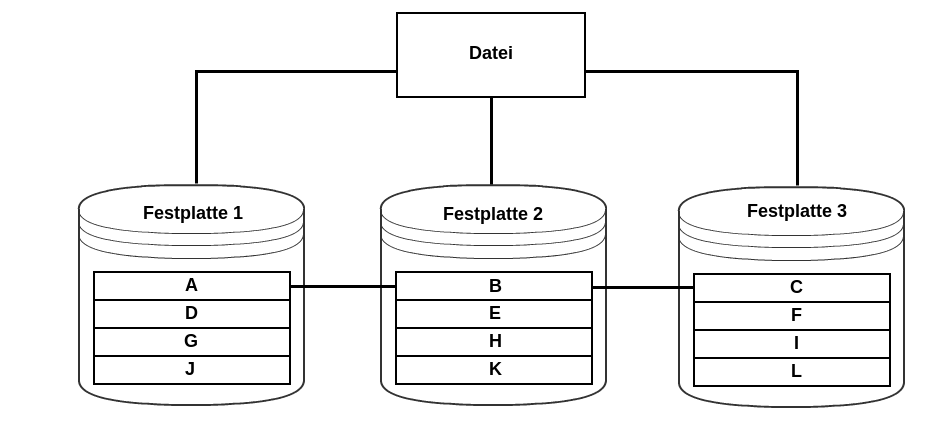
\includegraphics[scale=0.3]{resources/Bilder_Kapitel_2/RAID-0.png}
  \caption[Verteilung der Teilstücke einer Datei unter Verwendung von RAID-0]{Verteilung der Teilstücke einer Datei unter Verwendung von RAID-0 (In Anlehnung an \cite[Seite 279]{mandl08})}
  \label{fig-raid-0}
\end{figure}

Auf jede der drei Festplatten, in der Abbildung durch Festplatte 1, Festplatte 2 und Festplatte 3 dargestellt, werden verschiedene Teilstücke einer Datei, mit den Buchstaben A bis L dargestellt, gespeichert.
Daraus geht hervor, dass die Datei in mehrere Einzelstücke unterteilt und nicht redundant gespeichert wird.
Sollte eine Festplatte ausfallen, ist die gesamte Datei ungültig und nicht mehr brauchbar.

\subsection{RAID-1}
Bei einem \ac{RAID}-1-System werden alle Daten redundant auf die unterschiedlichen physikalischen Laufwerke gespeichert.
Sollte der \ac{RAID}-Verbund beispielsweise aus vier Festplatten bestehen, so wird eine Datei x auf allen vier Festplatten als Kopie abgelegt.
Das garantiert eine größere Ausfallsicherheit, da im Falle eines Defekts einer Festplatte, die Daten noch auf weiteren Platten verfügbar sind.
Dabei ist zu beachten, dass die Gesamtgröße der virtuellen Festplatte durch die kleinste verwendeten Platte festgelegt wird\cite[vgl.][Seite 281]{mandl13}.
Die Anzahl der Festplatten kann beliebig gewählt werden.
Je mehr Festplatten, desto größer die Ausfallsicherheit, wobei ein Benutzer immer den Kosten-Nutzen-Faktor abwägen muss.
Das bedeutet, sowohl die Kosten für eine Anschaffung steigen, als auch die Schreibzugriffe.
Ab einer gewissen Anzahl von Festplatten sinkt jedoch die Chance, dass alle zur gleichen Zeit ausfallen, auf einen vernachlässigbaren Prozentsatz.
Der Nachteil bei diesem Verfahren liegt im Schreibvorgang.
Dadurch, dass auf mehreren logischen Festplatten dieselbe Datei gespeichert werden muss, nimmt dies unter Umständen mehr Zeit in Anspruch als beim Beschreiben einer einzelnen Festplatte.
Jedoch kann je nach Einstellung der Lesevorgang beschleunigt werden, indem einzelne Sektoren der Datei von einzelnen Festplatten gelesen werden und später zusammengeführt werden\cite[vgl.][Seite 429 f.]{hert03}.
Dieses Verfahren wird in Abbildung \ref{fig-raid-1} aufgezeigt.

\begin{figure}[H]
  \centering
  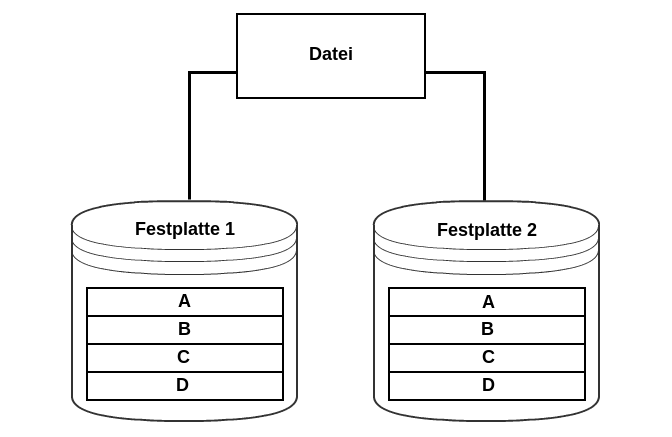
\includegraphics[scale=0.3]{resources/Bilder_Kapitel_2/RAID-1.png}
  \caption[Verteilung der Teilstücke einer Datei unter Verwendung von RAID-1]{Verteilung der Teilstücke einer Datei unter Verwendung von RAID-1 (In Anlehnung an \cite[Seite 280]{mandl08})}
  \label{fig-raid-1}
\end{figure}

Eine Datei wird auf zwei Festplatten, in der Abbildung durch Festplatte 1 und Festplatte 2 gekennzeichnet, gespeichert.
Obwohl zwei Festplatten verwendet werden, erhöht sich die Speicherkapazität nicht, da alle Teilstücke einer Datei, in der Abbildung als A bis D angegeben, gleichermaßen auf beide Festplatten verteilt werden.
Der Vorteil liegt jedoch in der Ausfallsicherheit.
Sollte eine der beiden Festplatten ausfallen, liegt eine Kopie der Datei immer noch auf der zweiten Festplatte, sodass der Benutzer der \ac{RAID}-1-Systems weiterhin Zugriff auf seine Daten hat.
Die defekte Festplatte müsste dann ausgetauscht und die Datei erneut kopiert werden.

\subsection{RAID-1+0}
Das \ac{RAID}-1+0 System, welches auch als \ac{RAID}-10 bezeichnet wird, kombiniert die Vorteile von \ac{RAID}-0 und \ac{RAID}-1-Systemen.
Für dieses Verfahren werden mindestens vier physikalische Festplatten benötigt\cite[vgl.][Seite 282]{mandl13}.
Jeweils 2 Platten werden dann als ein \ac{RAID}-0-Verbund zusammengeschlossen und die zwei daraus resultierenden logischen Festplatten als \ac{RAID}-1-Verbund\cite[vgl.][Seite 282]{mandl13}.
Somit ist eine Ausfallsicherheit gegeben, da Daten redundant gespeichert werden\cite[vgl.][Seite 282]{mandl13}.
Diese Verknüpfung der beiden \ac{RAID}-Systeme wird in Abbildung \ref{fig-raid-10} aufgezeigt.

\begin{figure}[H]
  \centering
  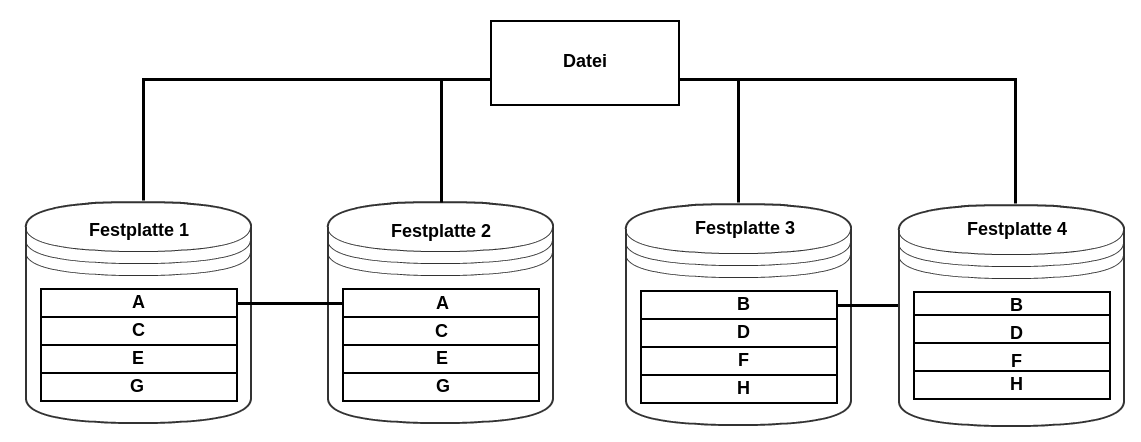
\includegraphics[scale=0.3]{resources/Bilder_Kapitel_2/RAID-10.png}
  \caption[Verteilung der Teilstücke einer Datei unter Verwendung von RAID-1+0]{Verteilung der Teilstücke einer Datei unter Verwendung von RAID-1+0 (In Anlehnung an \cite[Seite 281]{mandl08})}
  \label{fig-raid-10}
\end{figure}

Die Datei wird einerseits, wie bei einem \ac{RAID}-0-System, geteilt und der Speicherplatz somit vergrößert, andererseits werden die Daten auch redundant gespeichert, wie in einem \ac{RAID}-1-System.
Das Prinzip eines \ac{RAID}-1-Systems erkennt man in der Abbildung beispielhaft an Festplatte 2 und Festplatte 3.
Auch hier wird die Datei in Teilstücke von A bis H zerteilt und gespeichert.
Weiterhin kann man die redundante Speicherung eines \ac{RAID}-1-Systems an Festplatte 1 und Festplatte 2 erkennen.
Diese speichern beide dieselben Dateiinformationen, was bedeutet, dass bei einem Ausfall einer dieser Platten die Datei trotzdem verfügbar ist.
Somit sind die Vorteile beider Systeme in einem vereint.
Ein Benutzer vergrößert seinen Speicherplatz und erhält zugleich eine größere Ausfallsicherheit.
%
%   \subsection{Zusammenfassung}
%   \ac{RAID}-Systeme finden besonders bei Systemen mit hohen Datensicherheit oder großen Leistungsansprüchen anwendung.
%   Sollte auf eine hohe Ausfallsicherheit wert gelegt werden so empfiehlt sich das \ac{RAID}-1 System, da es Daten redundant speichert.
%   Wenn hingegen ein schneller Schreib- und Lesezugriff auf Daten gewährleistet werden soll, so sollte ein \ac{RAID}-0 System verwendet werden.
%   \ac{RAID}-1+0 vereint dabei beide Ansprüche, benötigt aber weitaus mehr Hardwareressourcen.
%   Sowohl das \ac{RAID}-0 als auch das \ac{RAID}-1 sind Verfahren, welche für die zu entwickelnde Anwendung in Betracht gezogen werden können.
%
